The output subsystem consists of a speaker and touchscreen, the speaker and touchscreen is the output for visual and audio. as it becomes the resultant of the raspberry pi os

\subsection{Layer Hardware}
Touchscreen,Speakers

\subsection{Layer Operating System}
Raspberry Pi OS

\subsection{Layer Software Dependencies}
N/A

\subsection{Speakers}
Speaker is for the audio output of the OS

\begin{figure}[h!]
	\centering
 	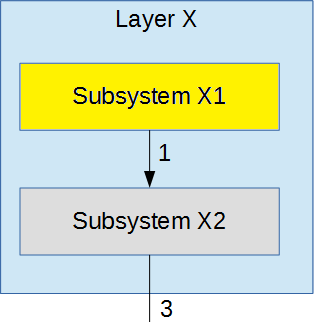
\includegraphics[width=0.60\textwidth]{images/subsystem}
 \caption{Example subsystem description diagram}
\end{figure}

\subsubsection{Subsystem Hardware}
Speaker is a Mini External USB Stereo Speaker

\subsubsection{Subsystem Operating System}
Raspberry pi os

\subsubsection{Subsystem Software Dependencies}
N/A

\subsubsection{Subsystem Programming Languages}
N/A

\subsubsection{Subsystem Data Structures}
N/A

\subsubsection{Subsystem Data Processing}
Signals from the OS create Audio for the speakers 


\subsection{Touch Screen}
Touch screen is used to show a visual display to the user

\begin{figure}[h!]
	\centering
 	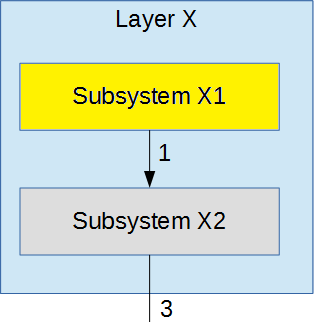
\includegraphics[width=0.60\textwidth]{images/subsystem}
 \caption{Example subsystem description diagram}
\end{figure}

\subsubsection{Subsystem Hardware}
7 inch LCD Display HDMI-compatible Touch Screen 1024x600 Resolution Capacitive Touch

\subsubsection{Subsystem Operating System}
Raspberry pi os

\subsubsection{Subsystem Software Dependencies}
N/A

\subsubsection{Subsystem Programming Languages}
N/A

\subsubsection{Subsystem Data Structures}
N/A

\subsubsection{Subsystem Data Processing}
Signals from the OS create visual display


 
